\section{Appendix}

  \subsection{Appendix A - Partnerships Objectives}
    \label{sec:AppendixA}
    \begin{figure}[H]
      \centering
      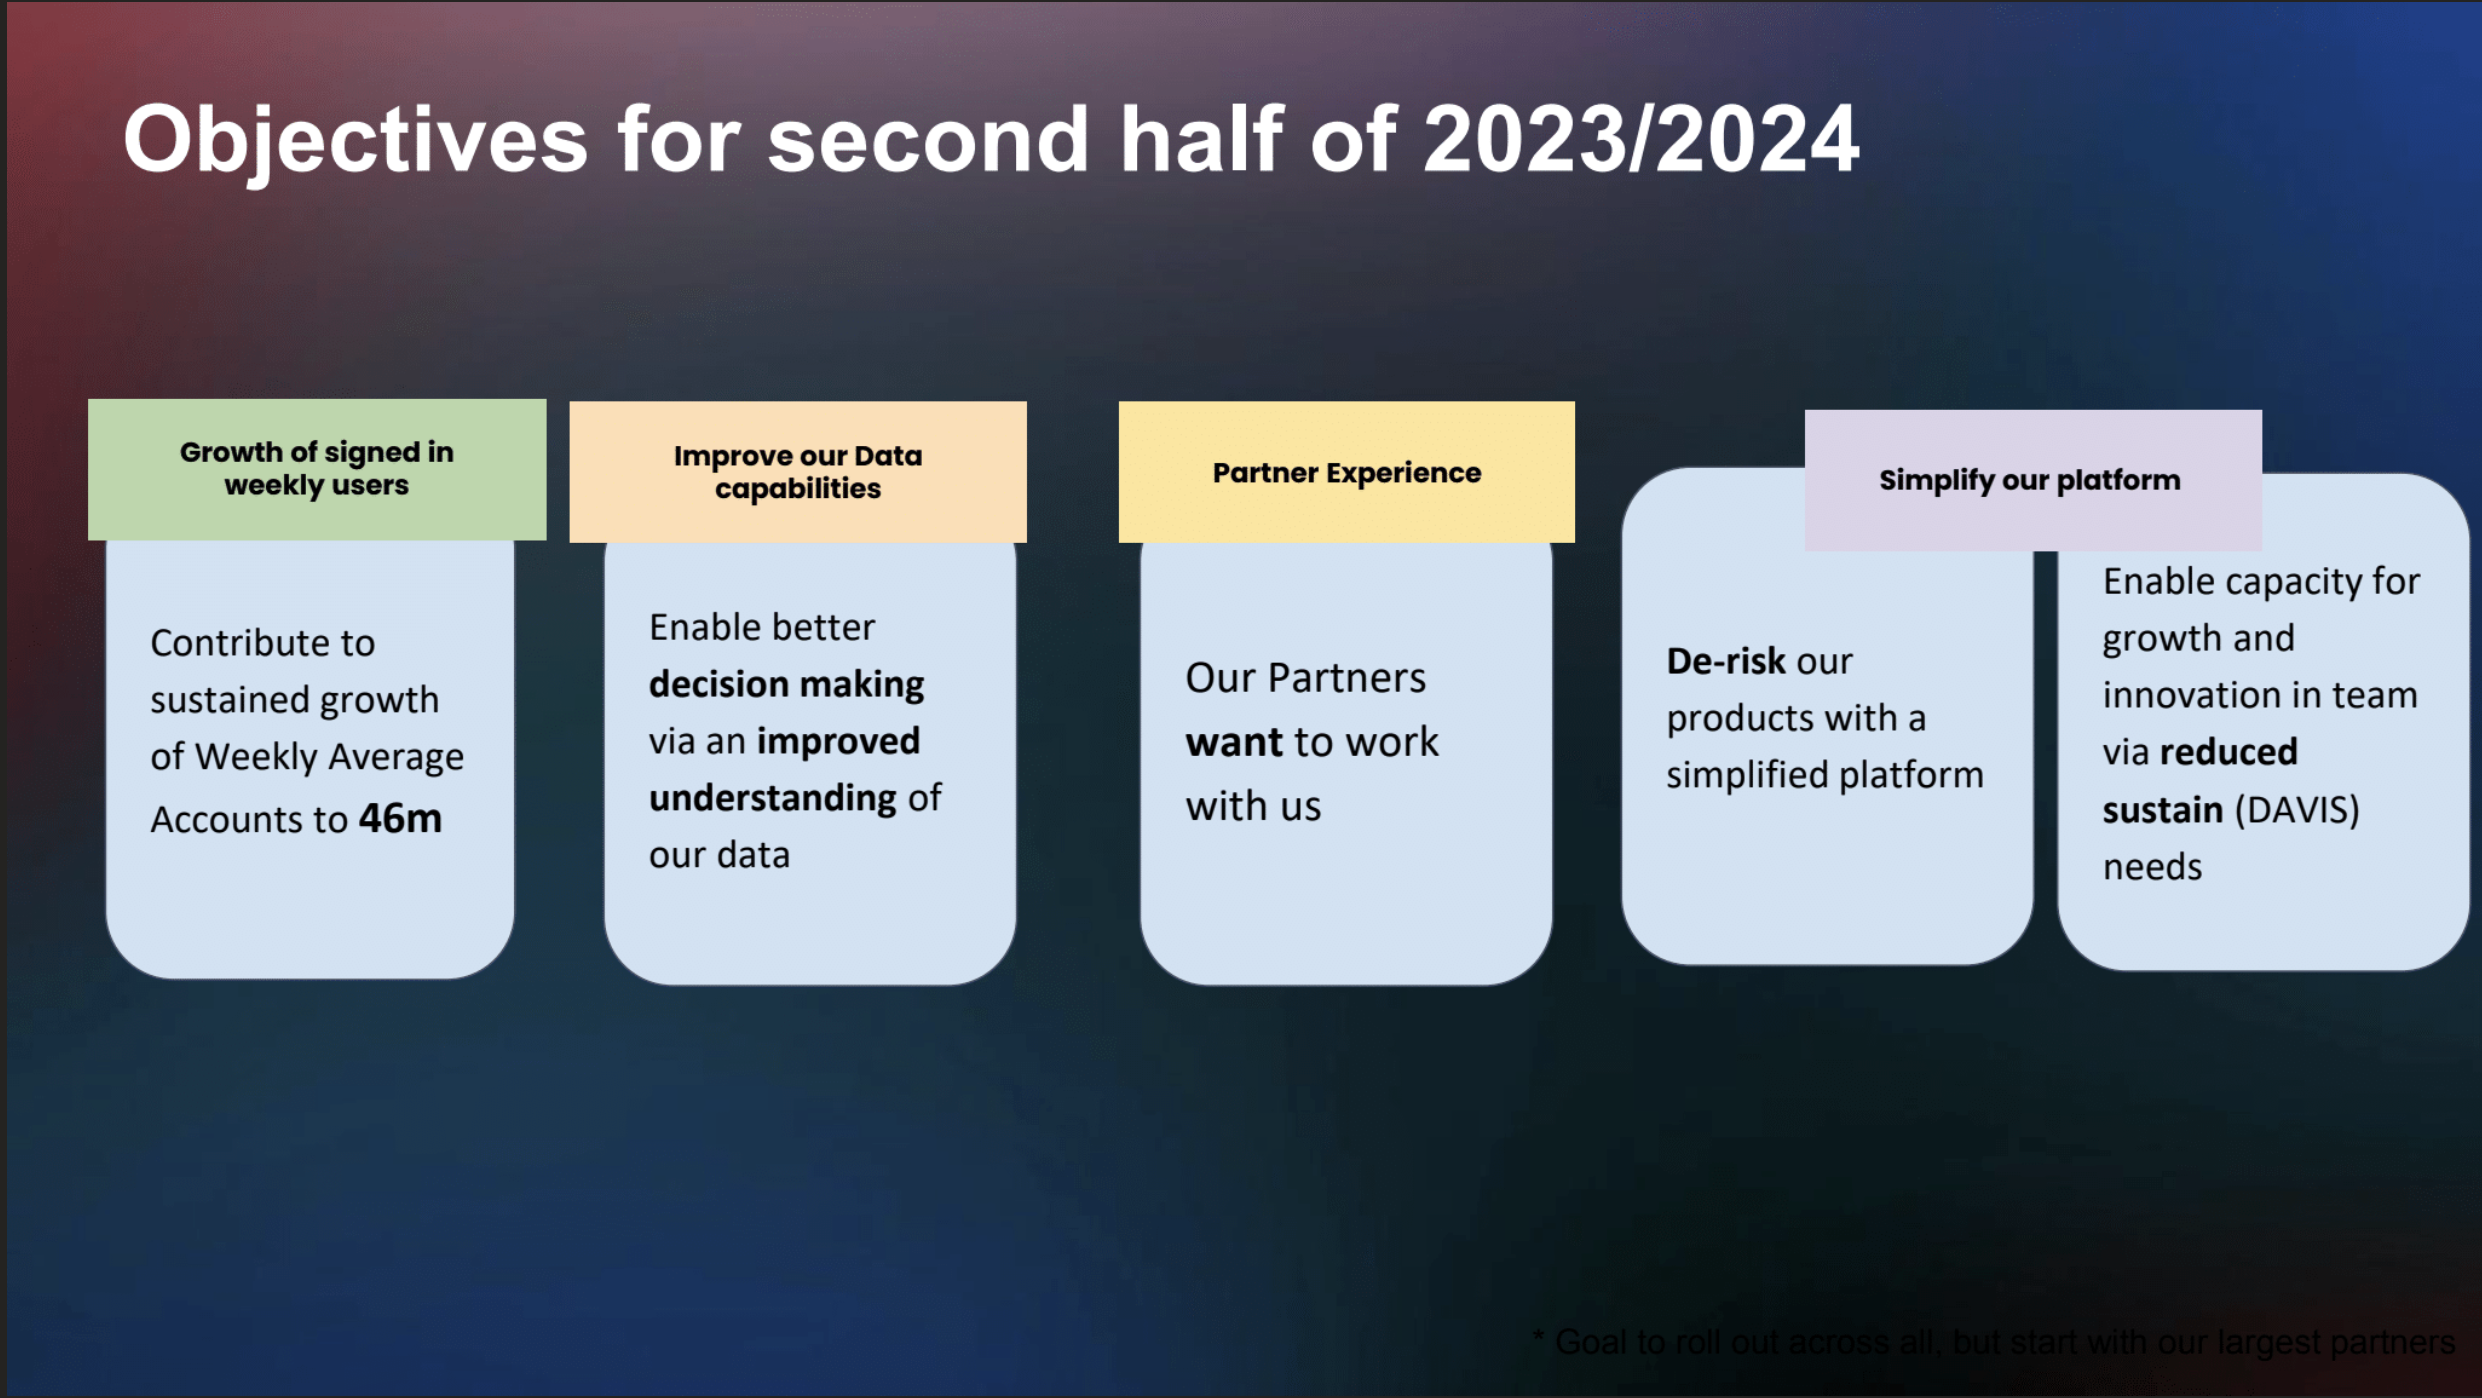
\includegraphics[width=12cm]{assets/appendix/partnershipsObjectives.png}
      \caption{Image taken from a presentation given at a partnership's context setting event (BBC Partnerships, 2023).}
      \label{fig:partnershipsObjectives}
    \end{figure}

  \newpage
  \subsection{Appendix B - Full schedules design including future external notification work}
    \label{sec:AppendixB}
    \begin{figure}[H]
      \centering
      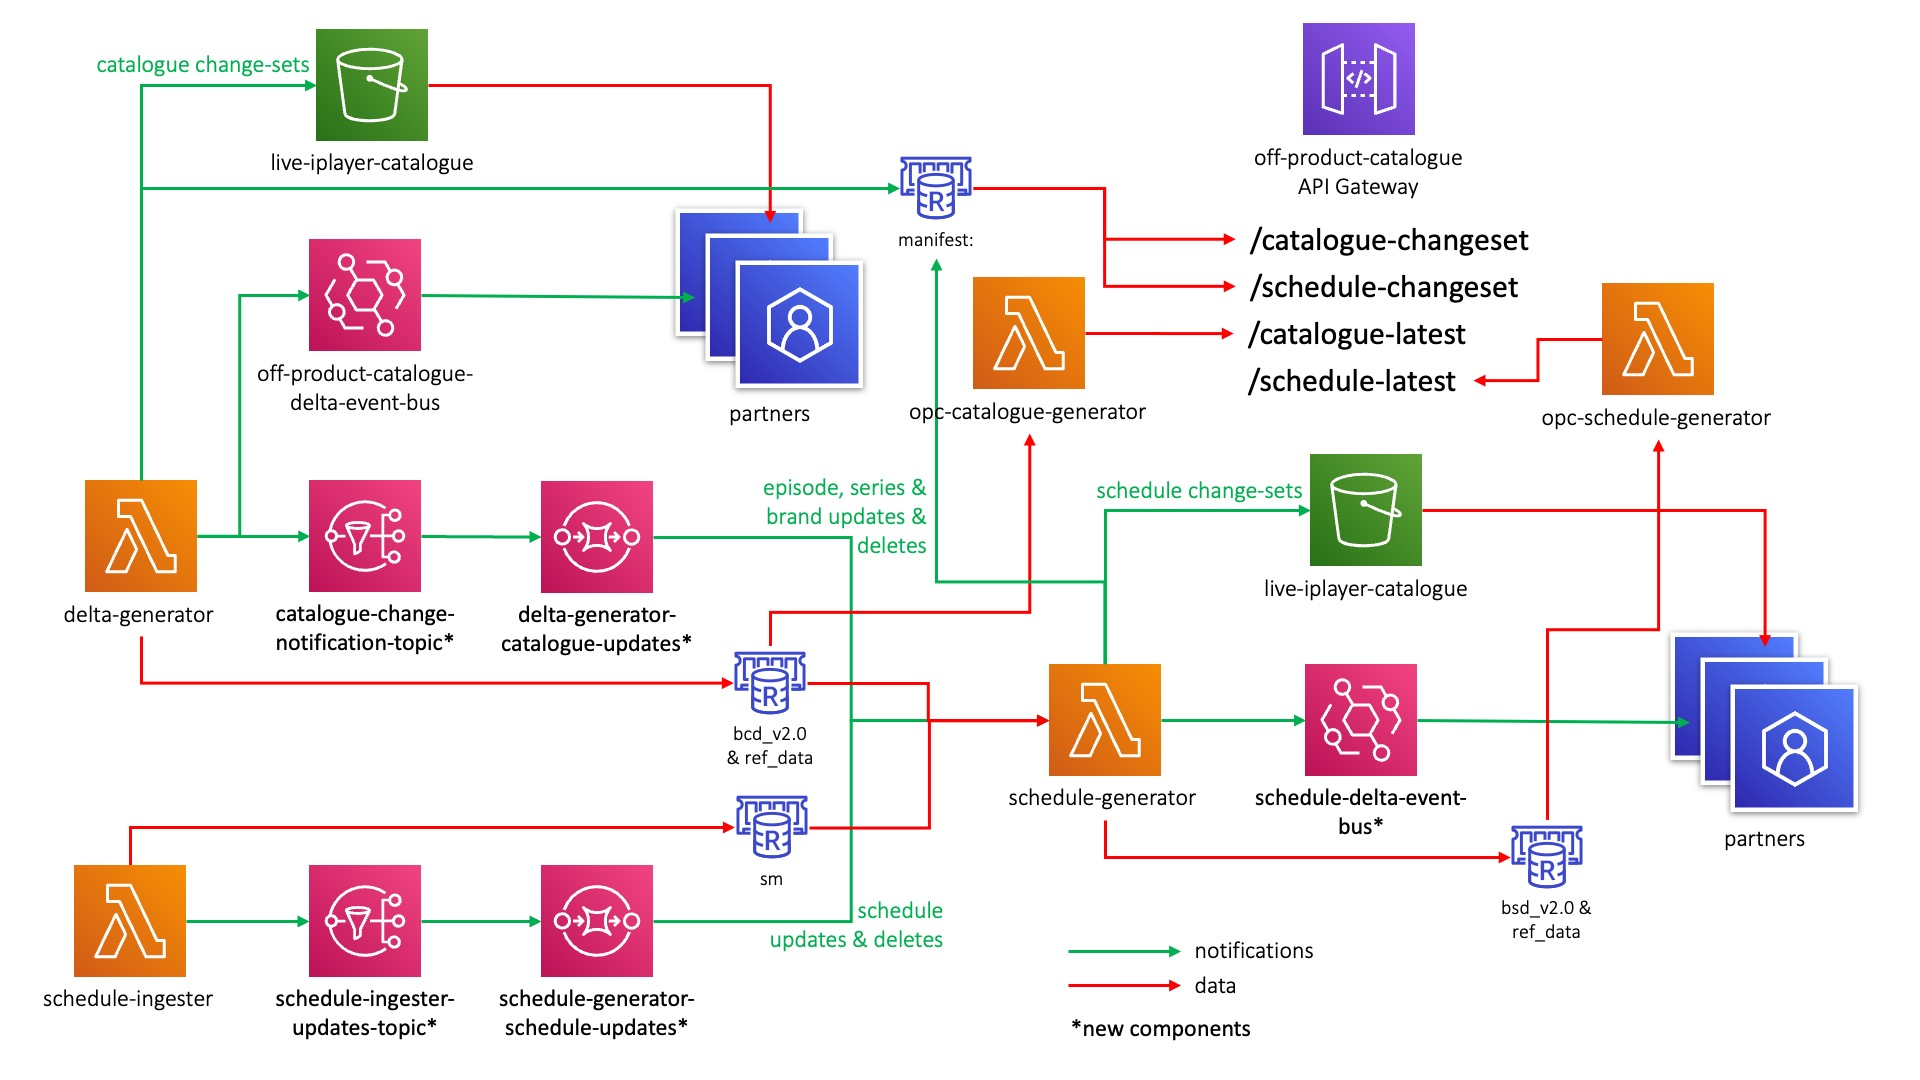
\includegraphics[width=12cm]{assets/appendix/initialDesign.jpg}
      \caption{Full diagram of design for schedules pipeline, including future notifications to partners work (Lloyd, 2023).}
      \label{fig:fullSpikeDesign}
    \end{figure}


  \newpage
  \subsection{Appendix C - Initial flow diagrams for how events would be processed}
    \label{sec:AppendixC}
    \begin{figure}[H]
      \centering
      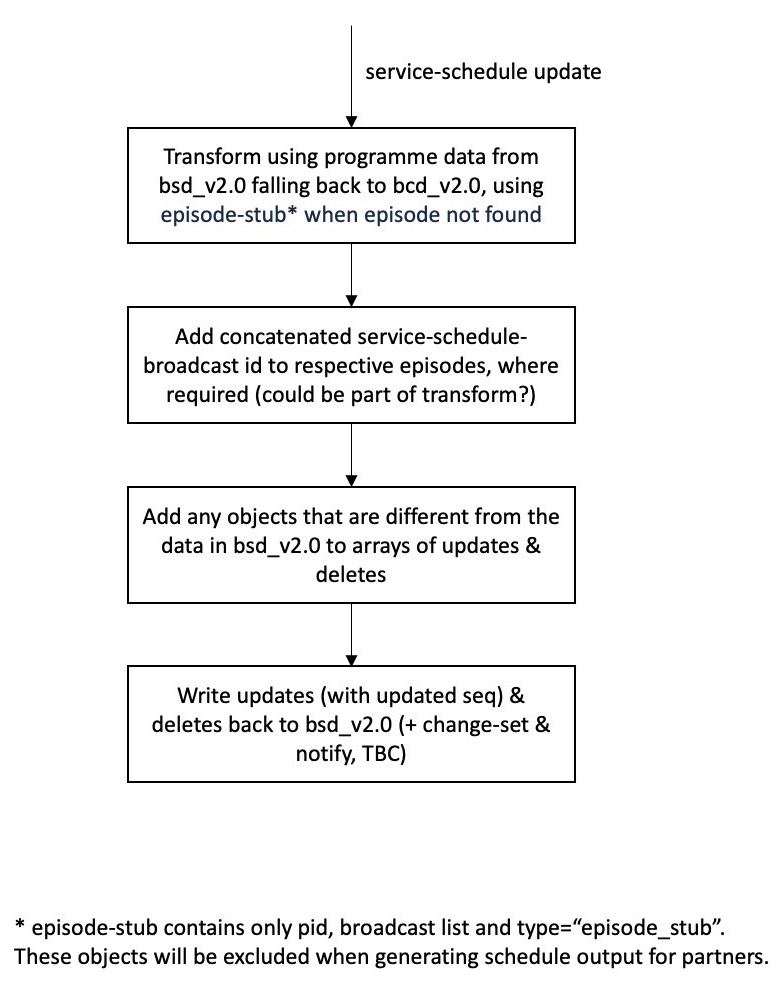
\includegraphics[width=6cm]{assets/initialDesign/scheduleUpdate.jpeg}
      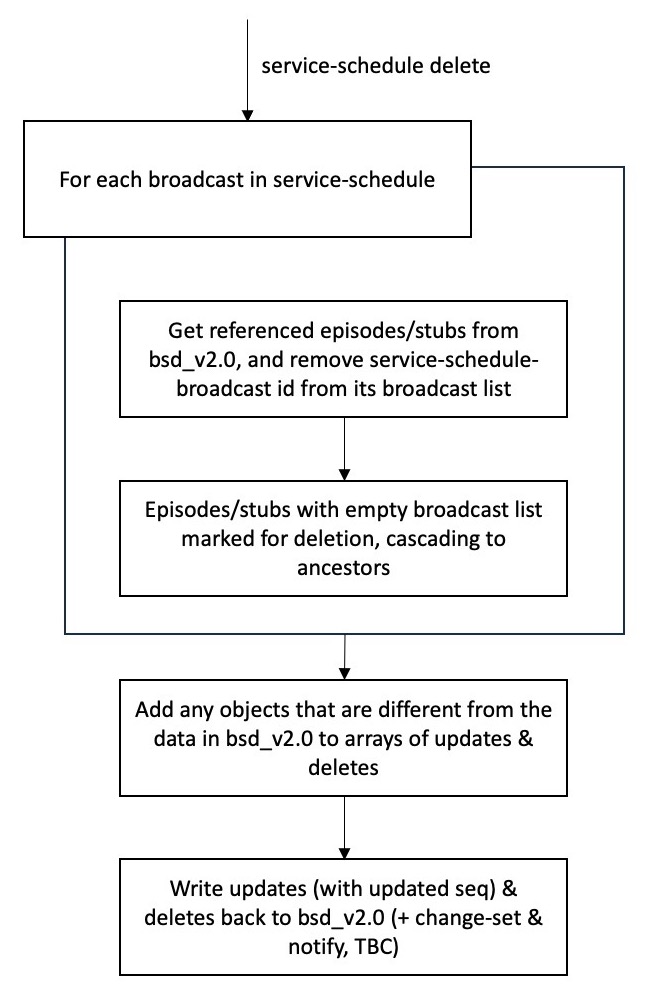
\includegraphics[width=6cm]{assets/initialDesign/scheduleDelete.jpeg}
      \caption{Flow diagrams for schedule events (Lloyd, 2023).}
      \label{fig:initialDesignSchedules}
    \end{figure}


    \begin{figure}[H]
      \centering
      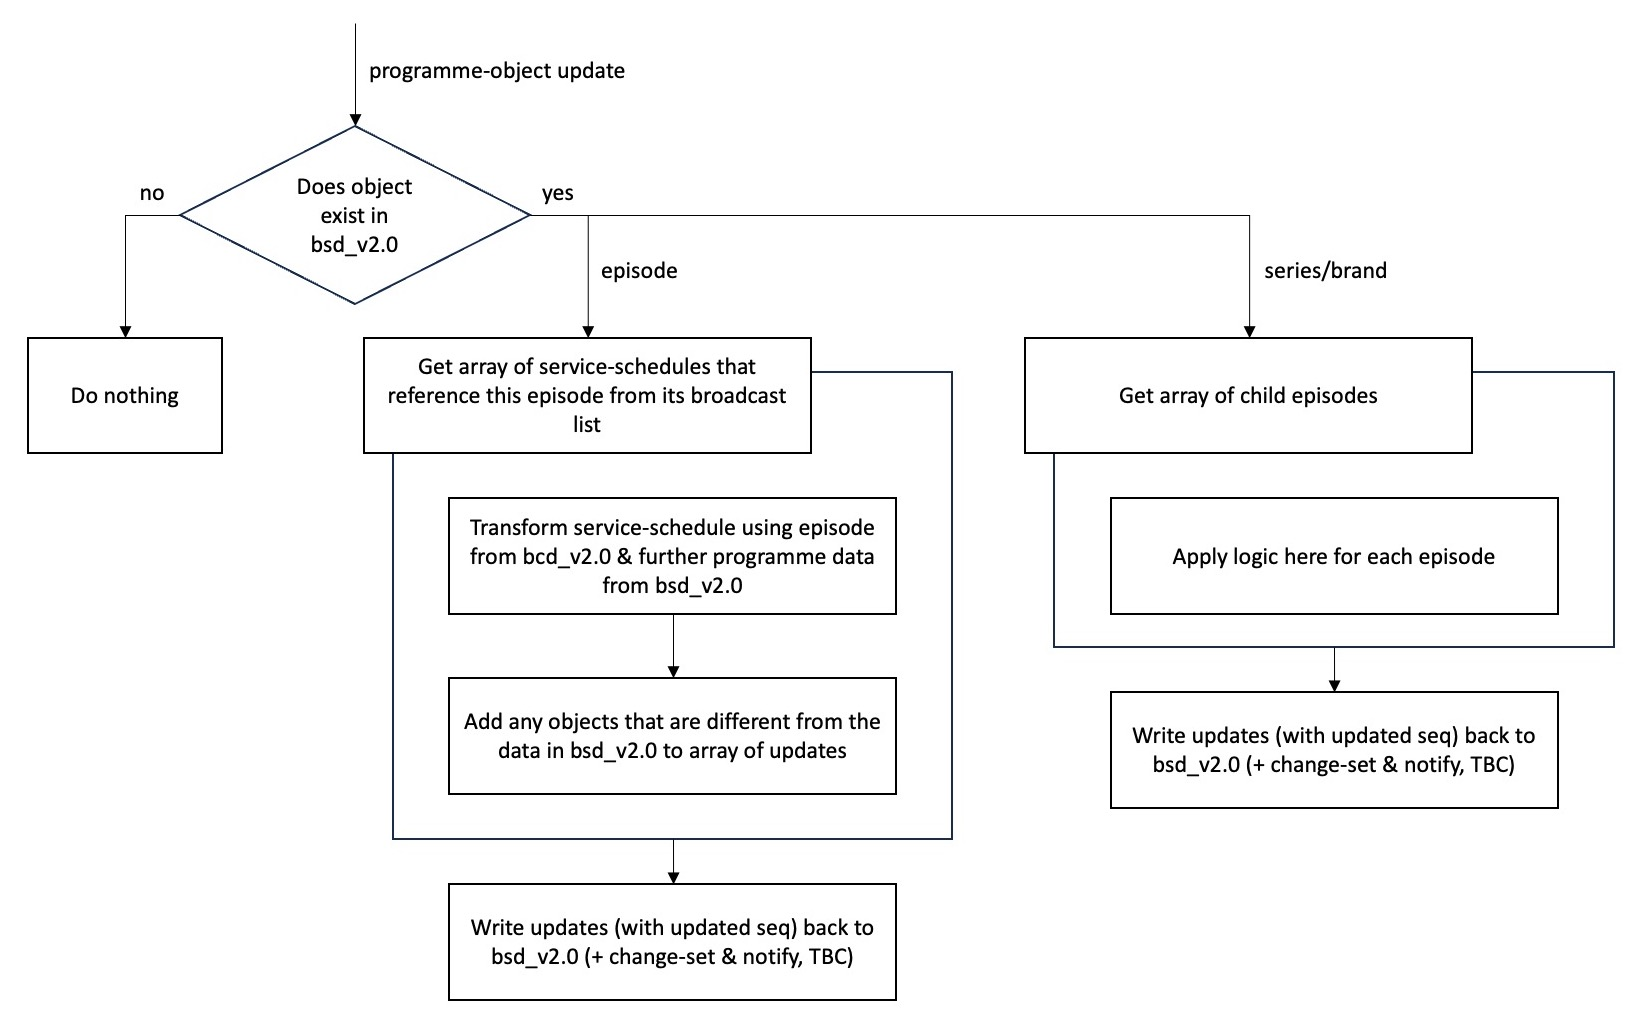
\includegraphics[width=12cm]{assets/initialDesign/programmeUpdate.jpg}
      \caption{Flow diagram for catalogue/programme events (Lloyd, 2023).}
      \label{fig:initialDesignProgrammes}
    \end{figure}

  
  \newpage
  \subsection{Appendix D - Full software spike document}
    \label{sec:AppendixD}
    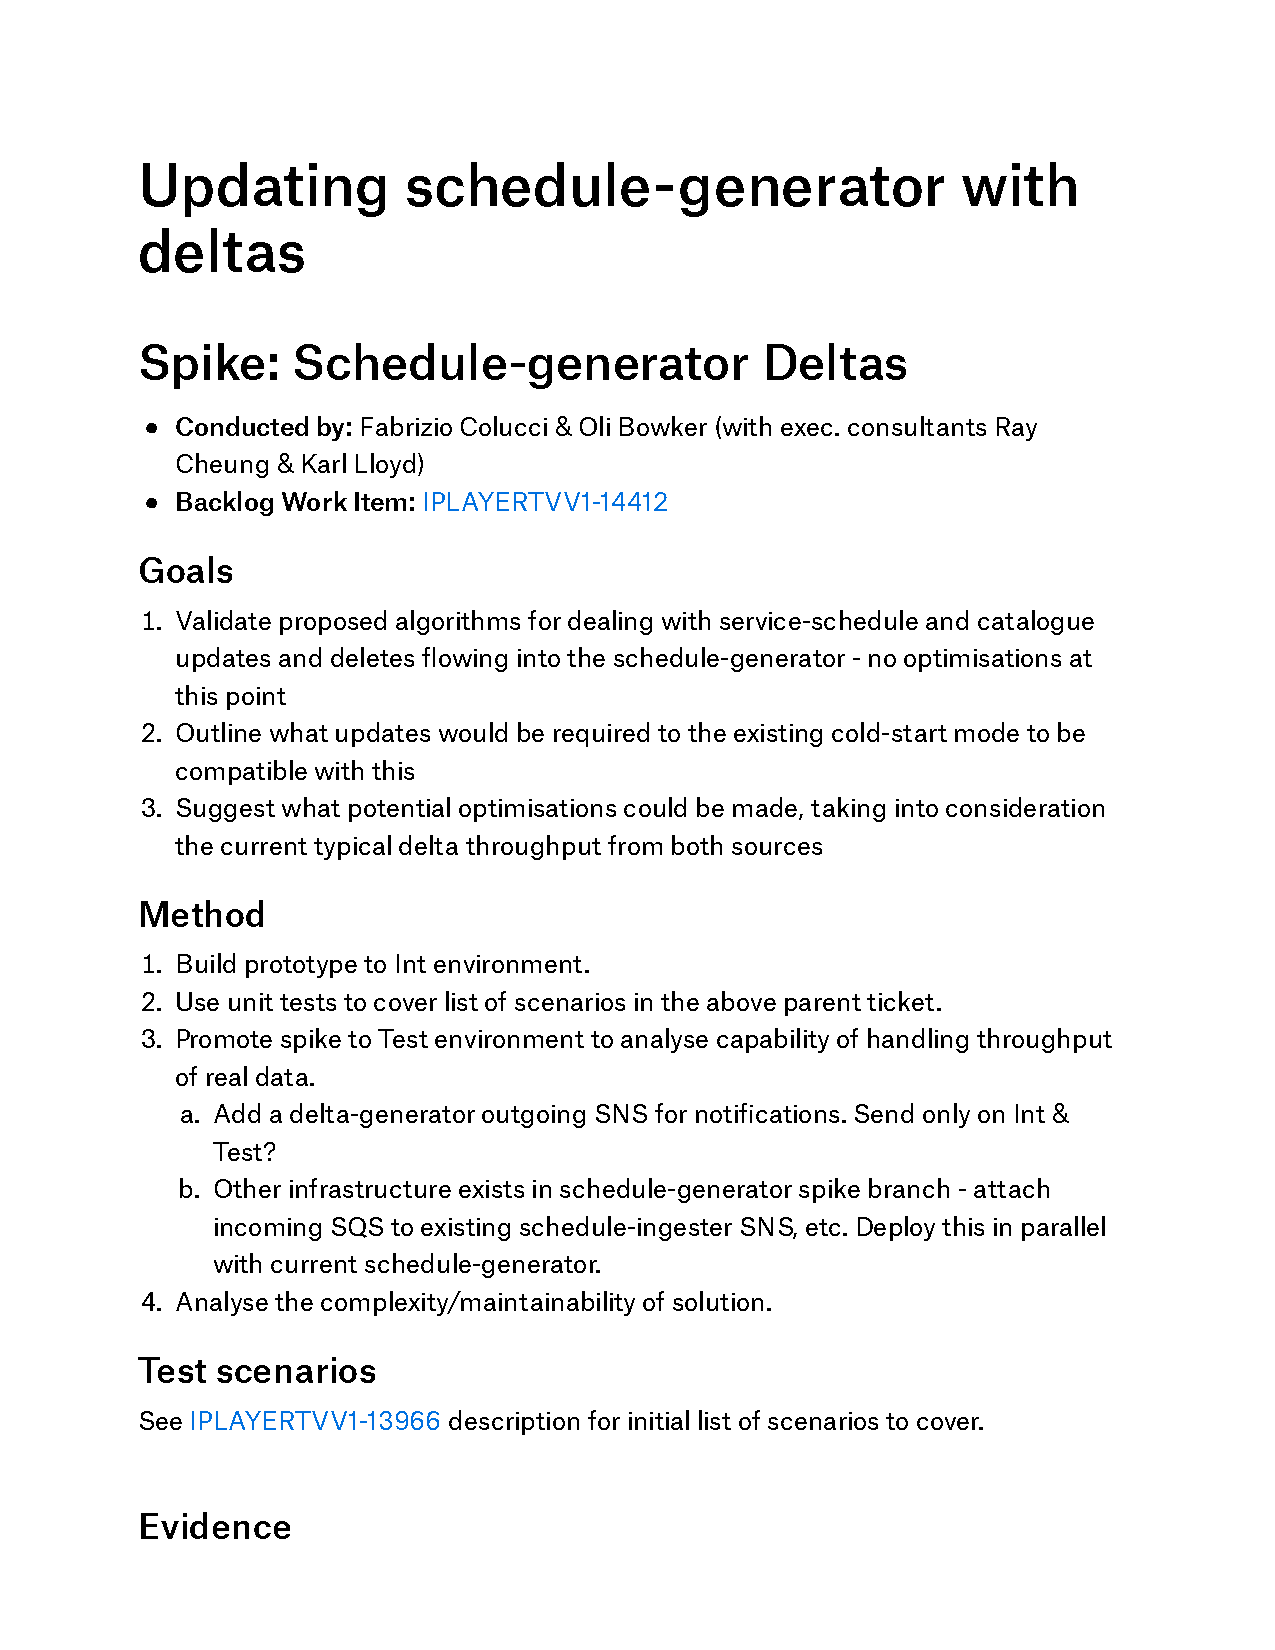
\includepdf[pages=-,scale=.6]{documents/spike.pdf}

  \newpage
  \subsection{Appendix E - Descriptions of Kanban stages used by SpaceChimp}
    \label{sec:AppendixE}

    \begin{itemize}
      \item \textbf{Ready for dev} - Tasks that are ready to be picked up for development.
      \item \textbf{Kick-off} - Tasks that need a test kick-off, which is not the same as the previous sections kick-off. This is where developers
      discuss the task with a member of the test team and determine the Acceptance Criteria (ACs) and test approach for the task.
      \item \textbf{In Progress} - Tasks that are being developed and worked on, this includes when code is being reviewed by other developers.
      \item \textbf{In Test} - Task has been completed and changes are on the test environment. A member of the test team can now test the ticket
      based on the previous discussions had in the kick-off. If things have changed during development, an additional hand-over with the test team 
      is done to discuss the new changes.
      \item \textbf{Releasing} - After a ticket task has been tested and has met the specified ACs, the task is moved to the releasing column signifying 
      that is ready to be deployed to the live environment.
      \item \textbf{Live monitoring} - Tasks in this column need to be monitored on the live environment to make sure that the change is functioning as expected.
    \end{itemize}
    

  \newpage
  \subsection{Appendix F - Architectural decision for single schedules store}
  \label{sec:AppendixF}

  \subsection*{Architecture Decision Record 022: Single source for schedule data}

  \subsubsection*{Context}
  Schedule documents rely on catalogue data for titling, programme descriptions, subtitling and viewer discretion data. When requesting 
  schedules via the API Gateway the partner also receives episode, series and brand data associated with the schedules requested as part of
  the response. This data can be retrieved from the catalogue redis store but the schedules pipeline is then fully reliant on the catalogue pipeline.
  This reliance of the catalogue pipeline (\emph{{bcd\_v2.0}:}) means that the schedule API gateway is not independent therefore it was requested to make 
  catalogue data more integrated within the schedule redis stores. This ADR describes the decision made to ensure data independence.
  \subsubsection*{Decision}
  Copy over all catalogue data currently relating to schedules into the keyspace \emph{{bsd\_v2.0}:} and \emph{{bsd\_v2.0\_ref\_data}:} respectively on 
  notification events or coldstart. This ensures the API Gateway can retrieve all of its information from one source and keep it's integrity and
  self-consistency. This data should also be removed when no longer referenced by any schedules.

  \subsubsection*{Status}
  Accepted

  \subsubsection*{Consequences}
    \begin{itemize}
      \item Overhead of copying over data existing data.
      \item Added maintenance and code complexity.
      \item Potential synchronisation issue when copying/deleting data across redis stores.
    \end{itemize}


  \newpage
  \subsection{Appendix G - Burn-ups created through the projects life-cycle}
    \label{sec:AppendixG}

    \begin{figure}[H]
      \centering
      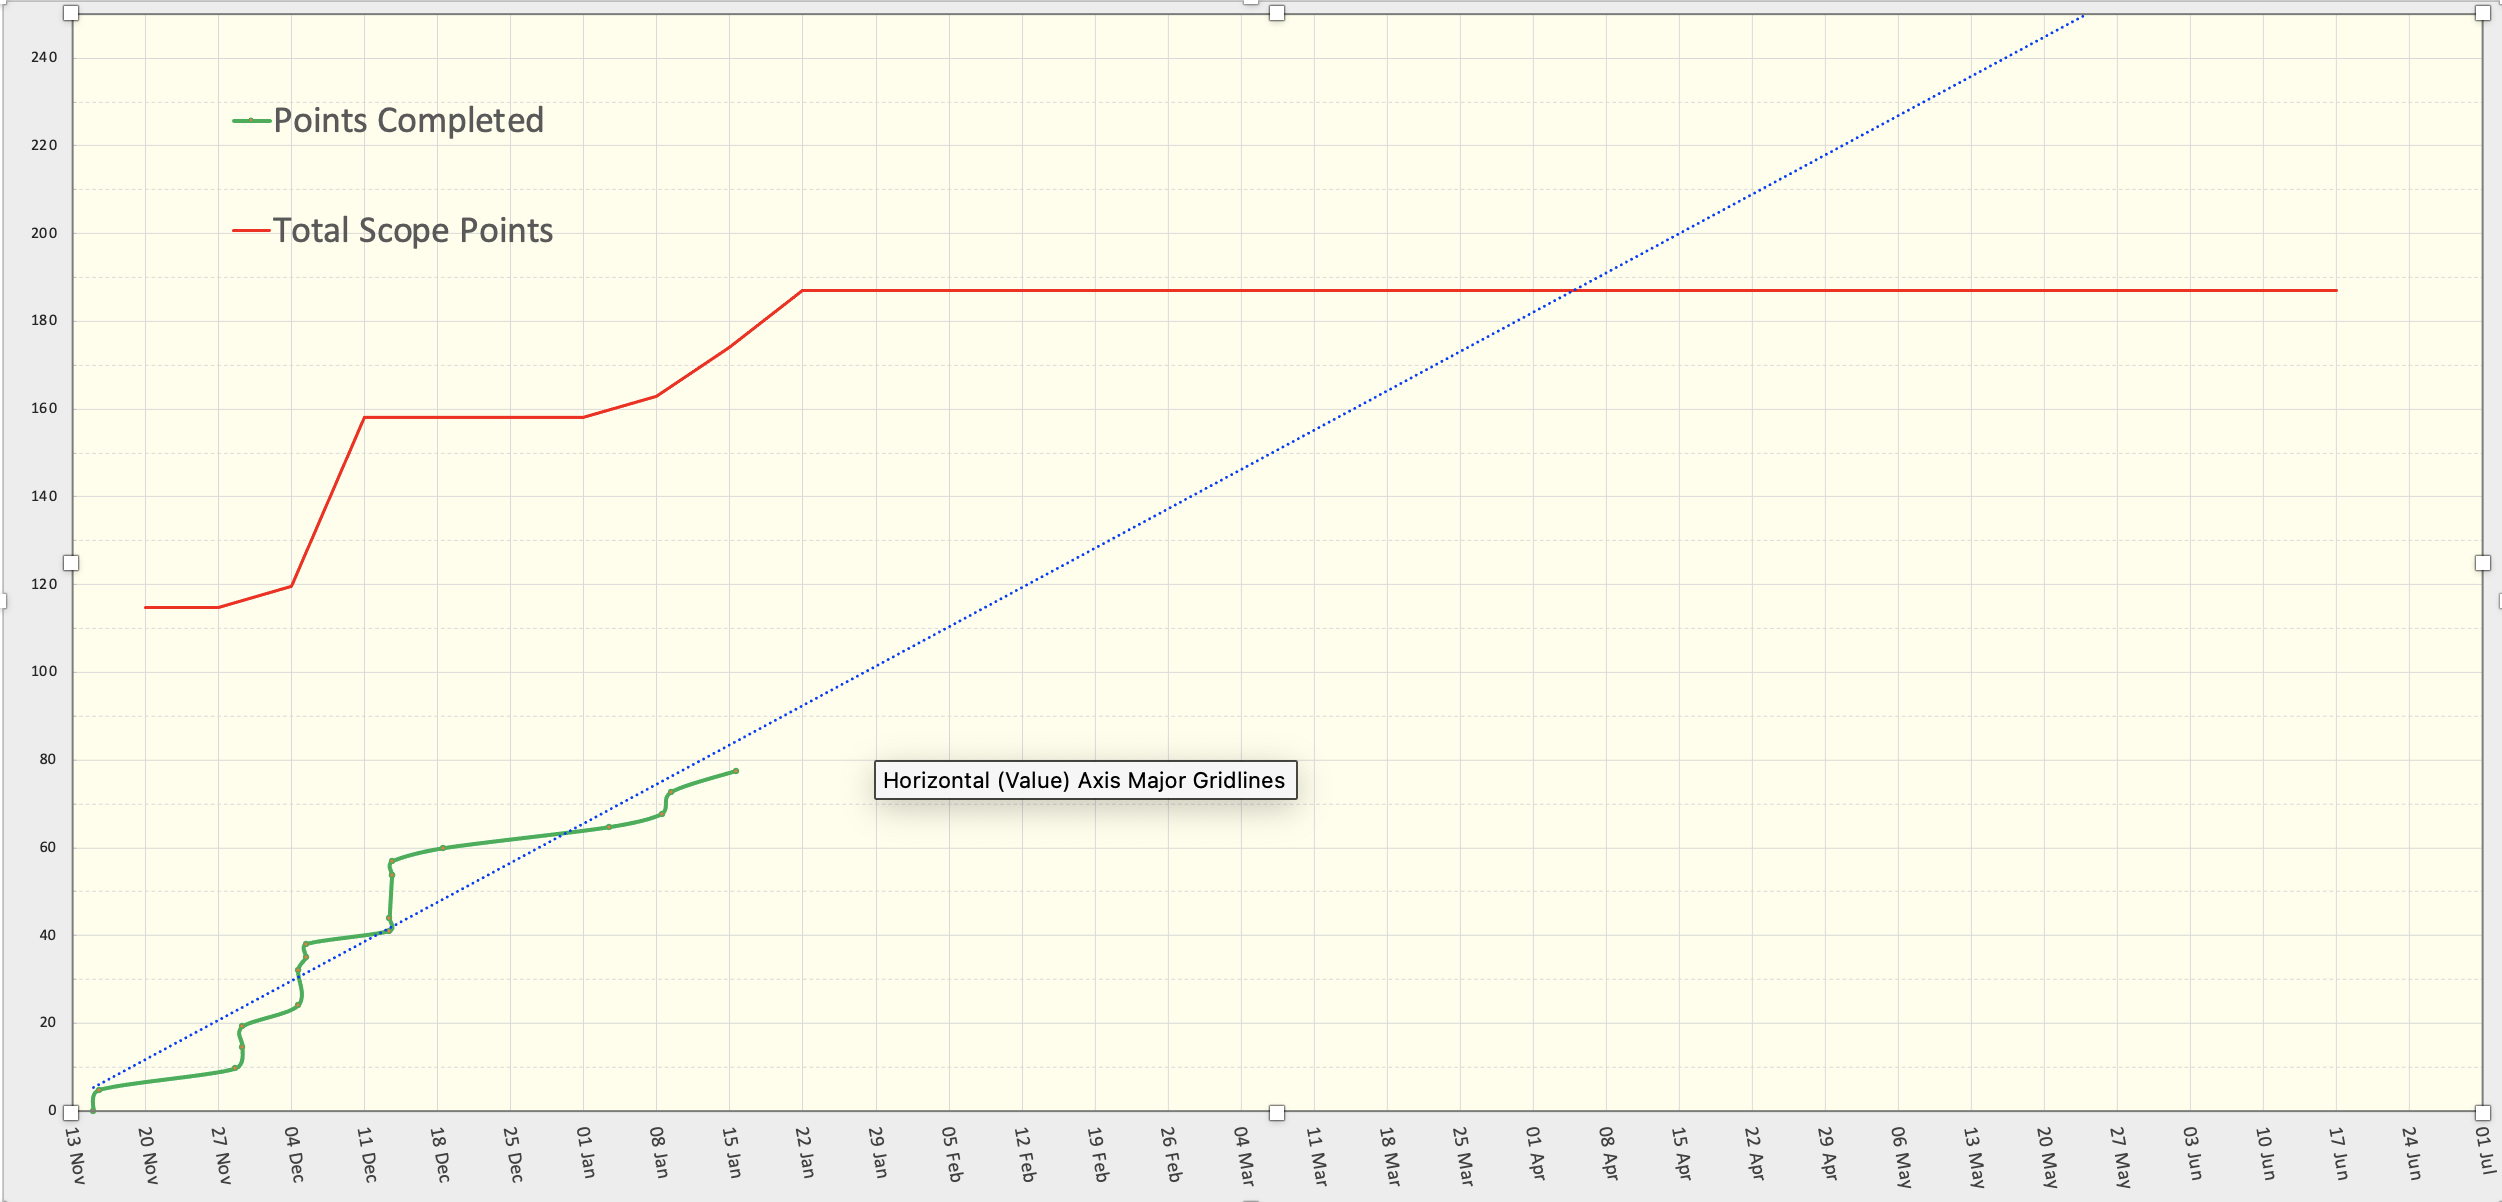
\includegraphics[width=12cm]{assets/outputs/burnups/01-16.png}
      \caption{Burn-up chart January 16th.}
      \label{fig:burnup1}
    \end{figure}
  
    \begin{figure}[H]
      \centering
      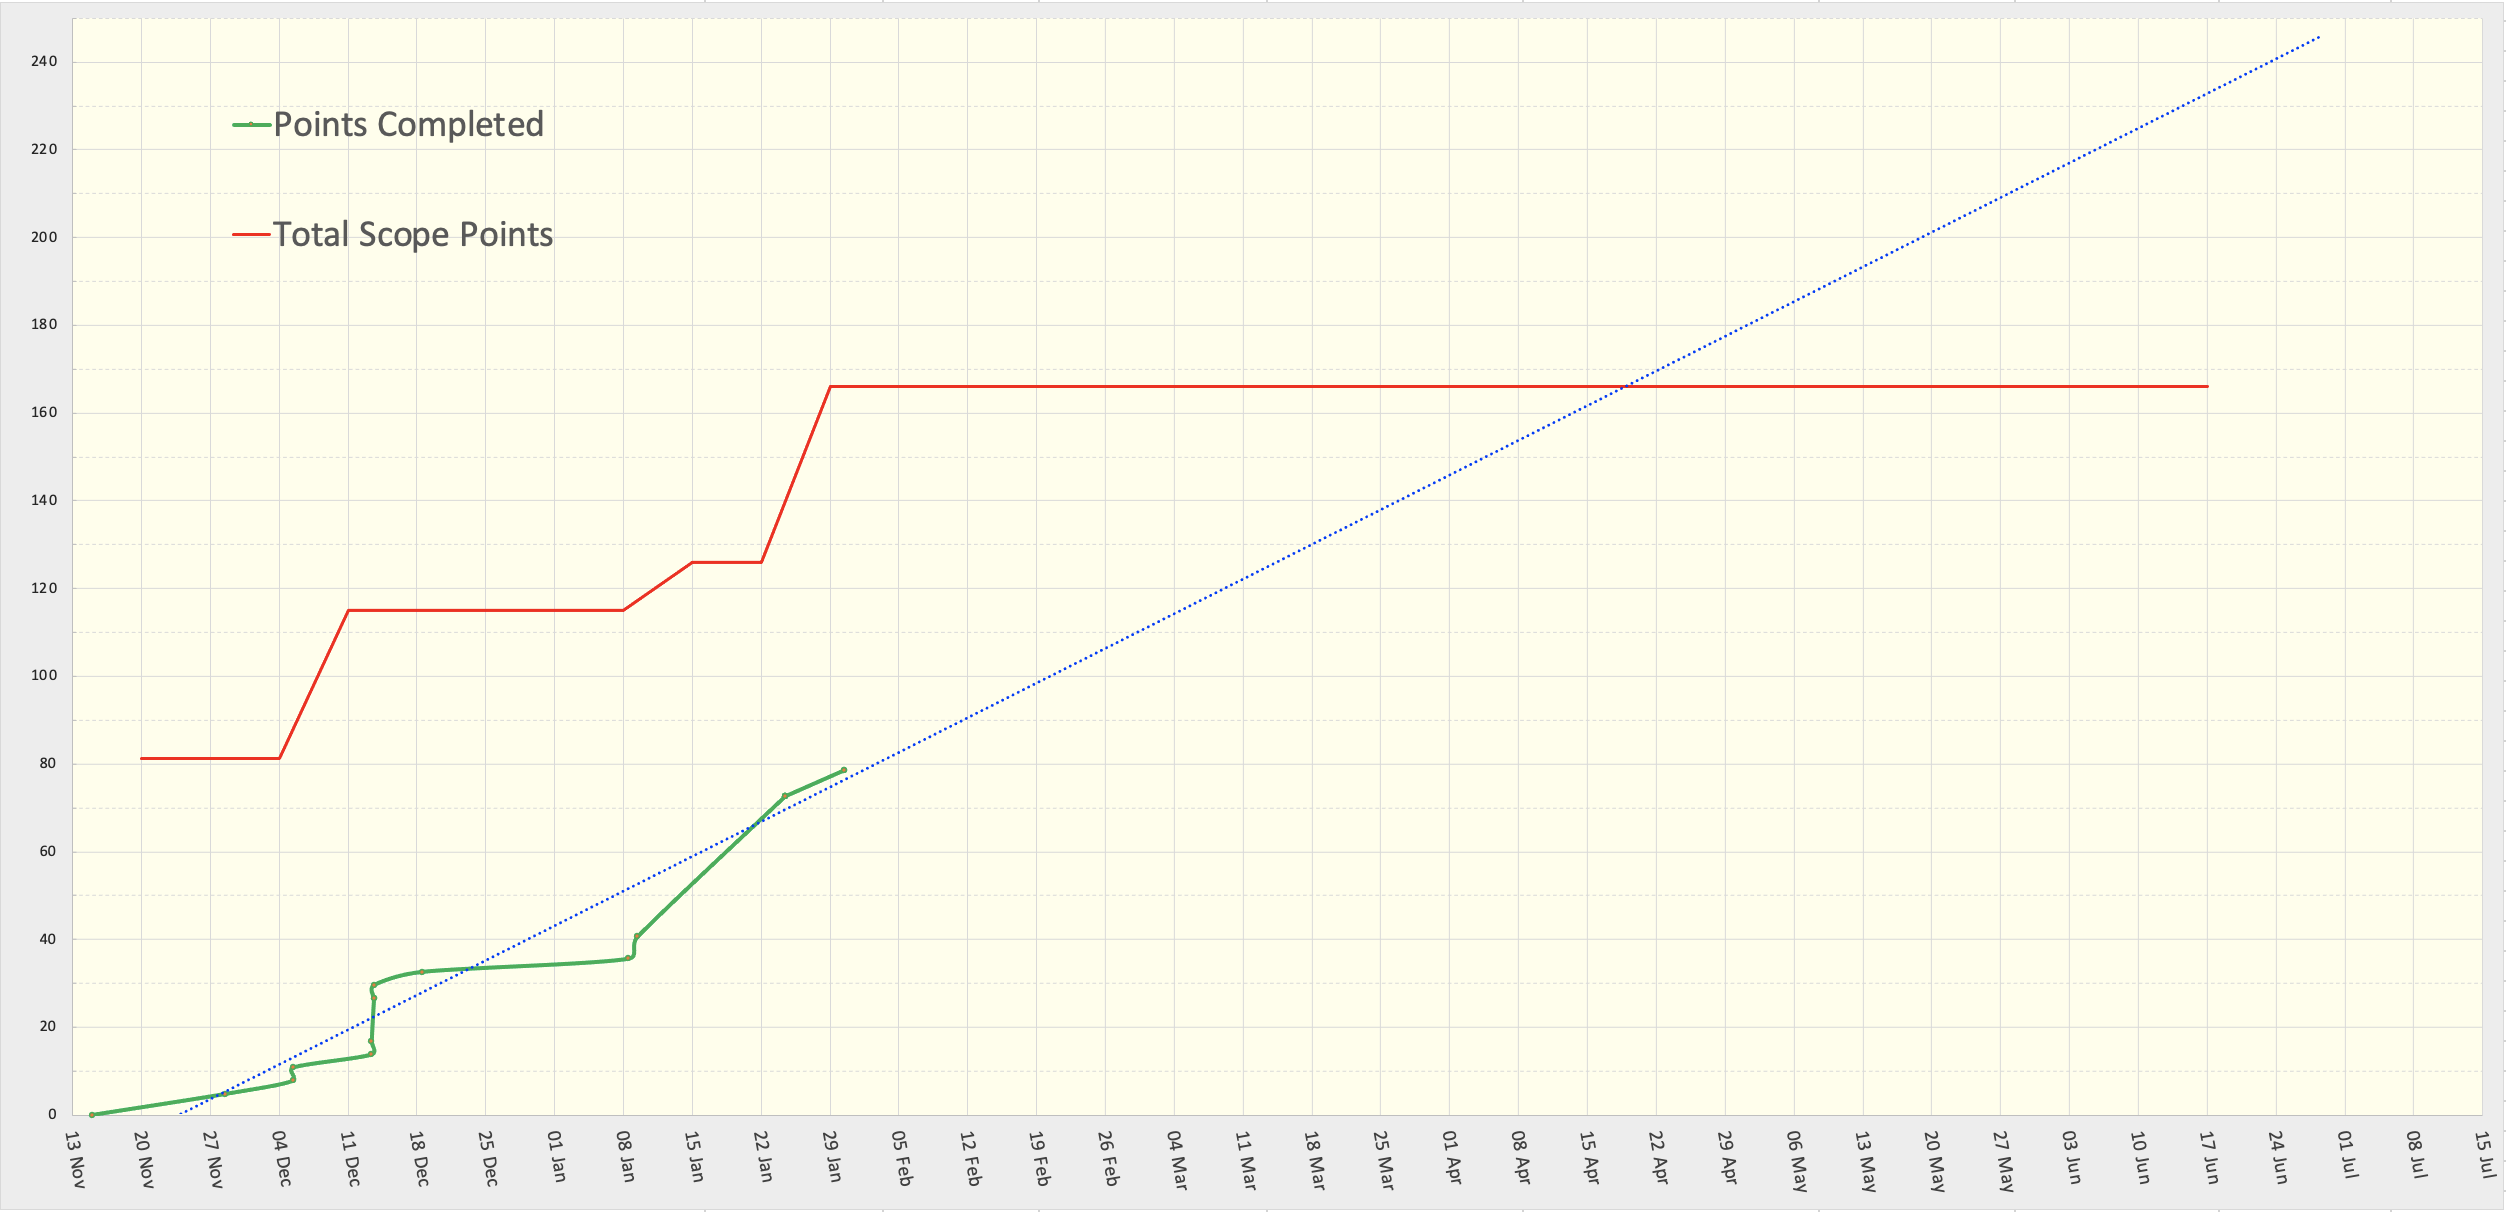
\includegraphics[width=12cm]{assets/outputs/burnups/01-30.png}
      \caption{Burn-up chart January 30th.}
      \label{fig:burnup2}
    \end{figure}
  
    \begin{figure}[H]
      \centering
      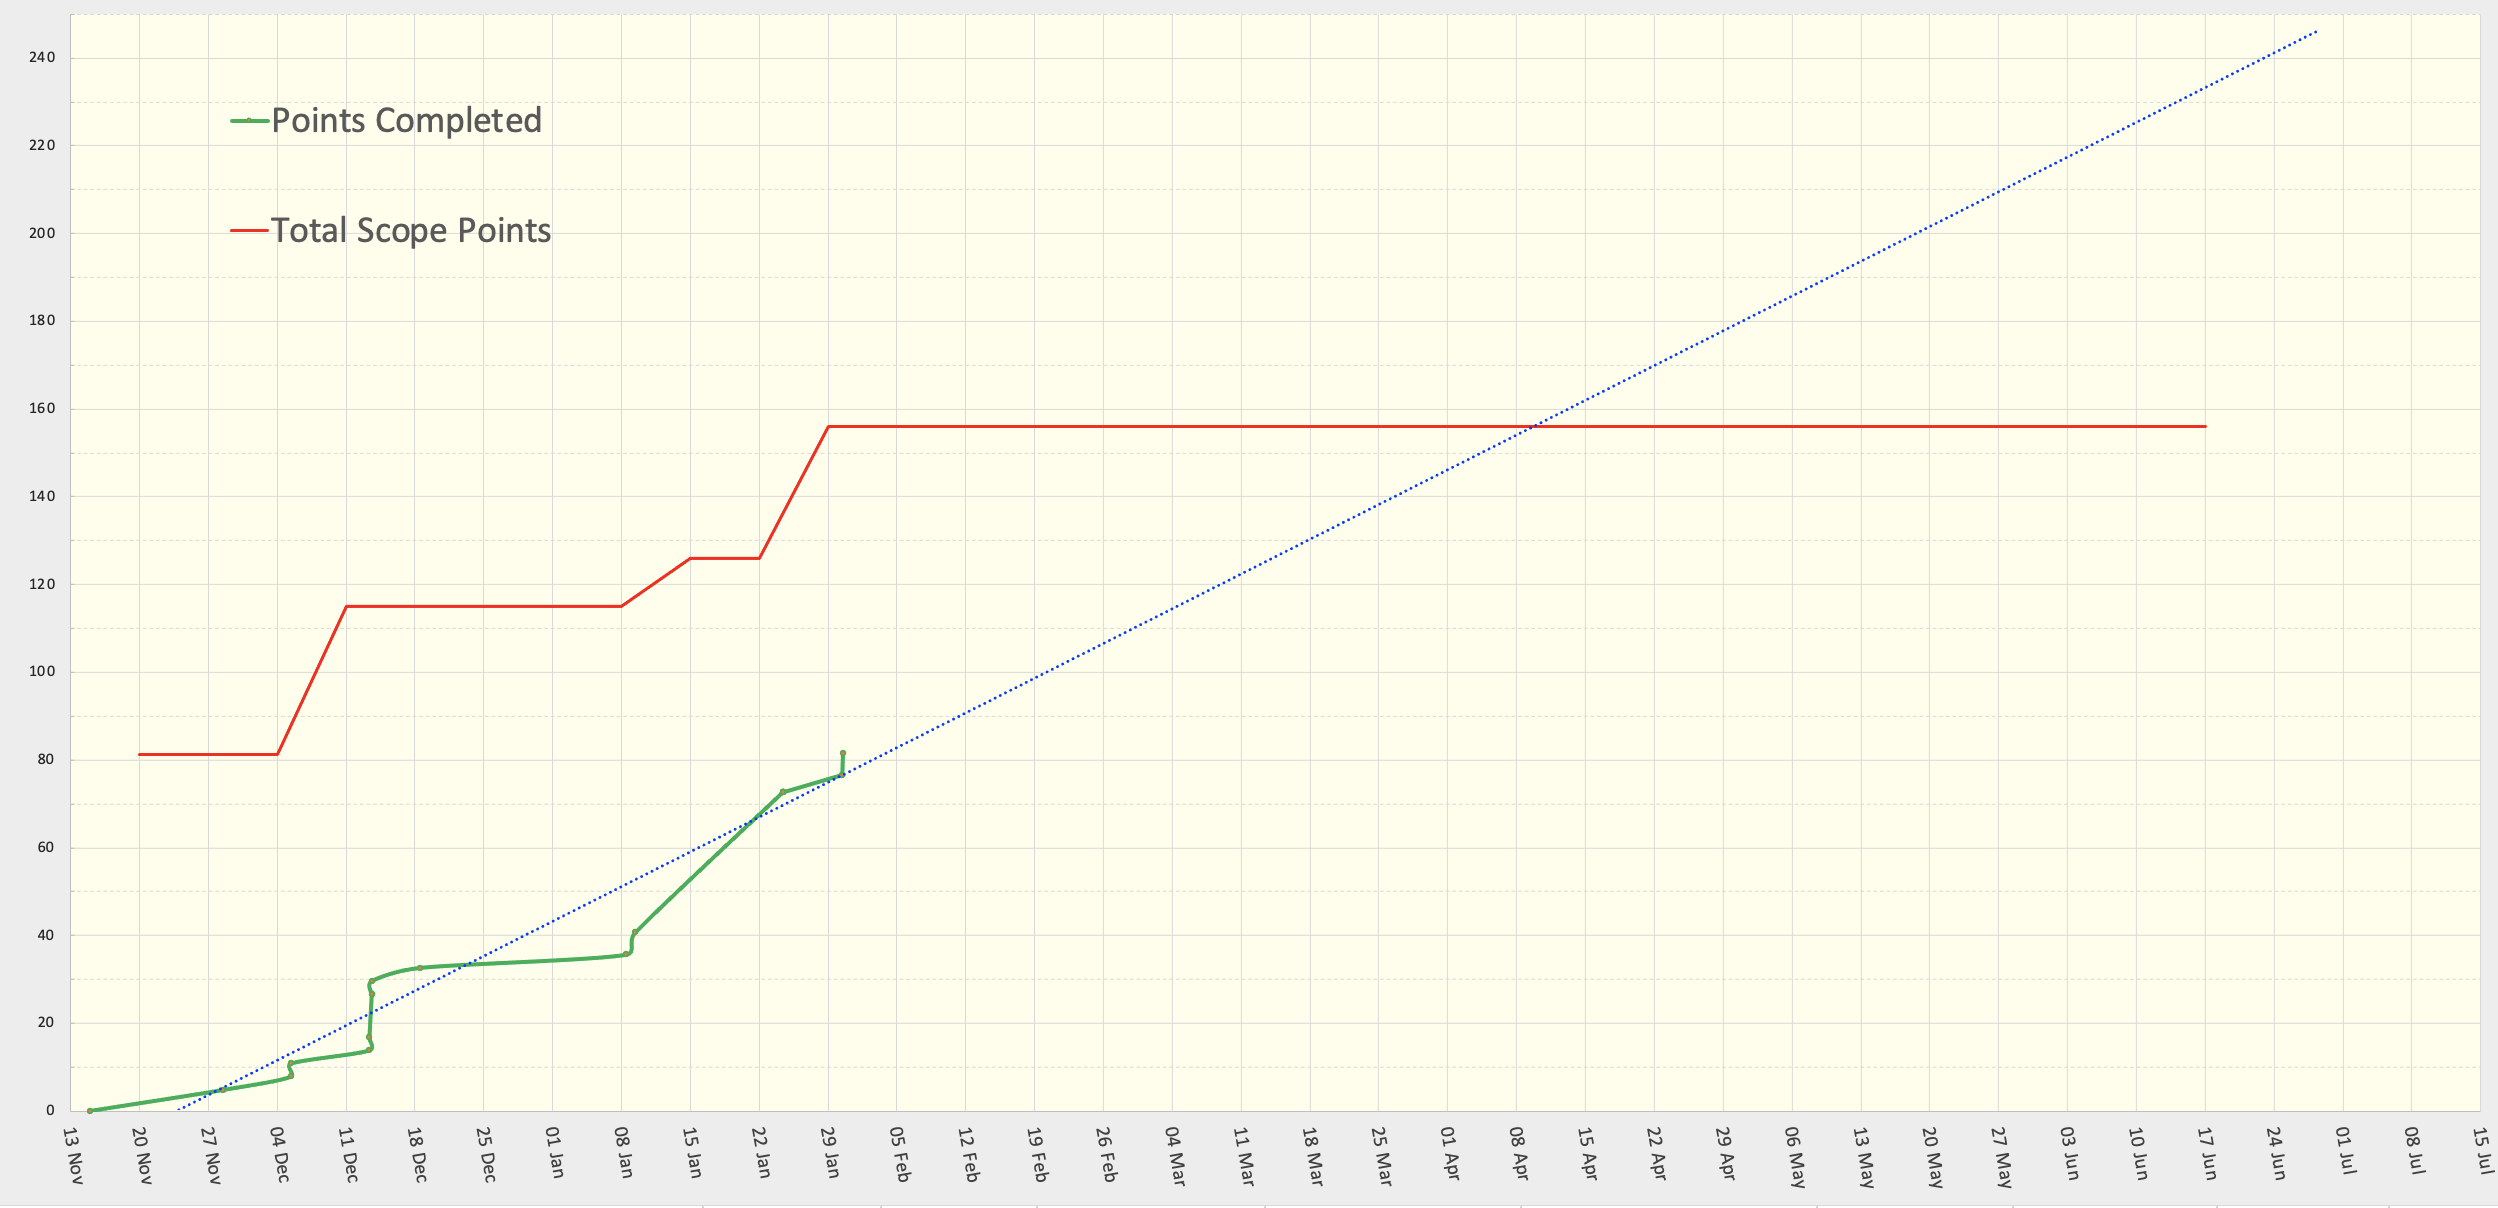
\includegraphics[width=12cm]{assets/outputs/burnups/02-05.png}
      \caption{Burn-up chart February 5th.}
      \label{fig:burnup3}
    \end{figure}
  
    \begin{figure}[H]
      \centering
      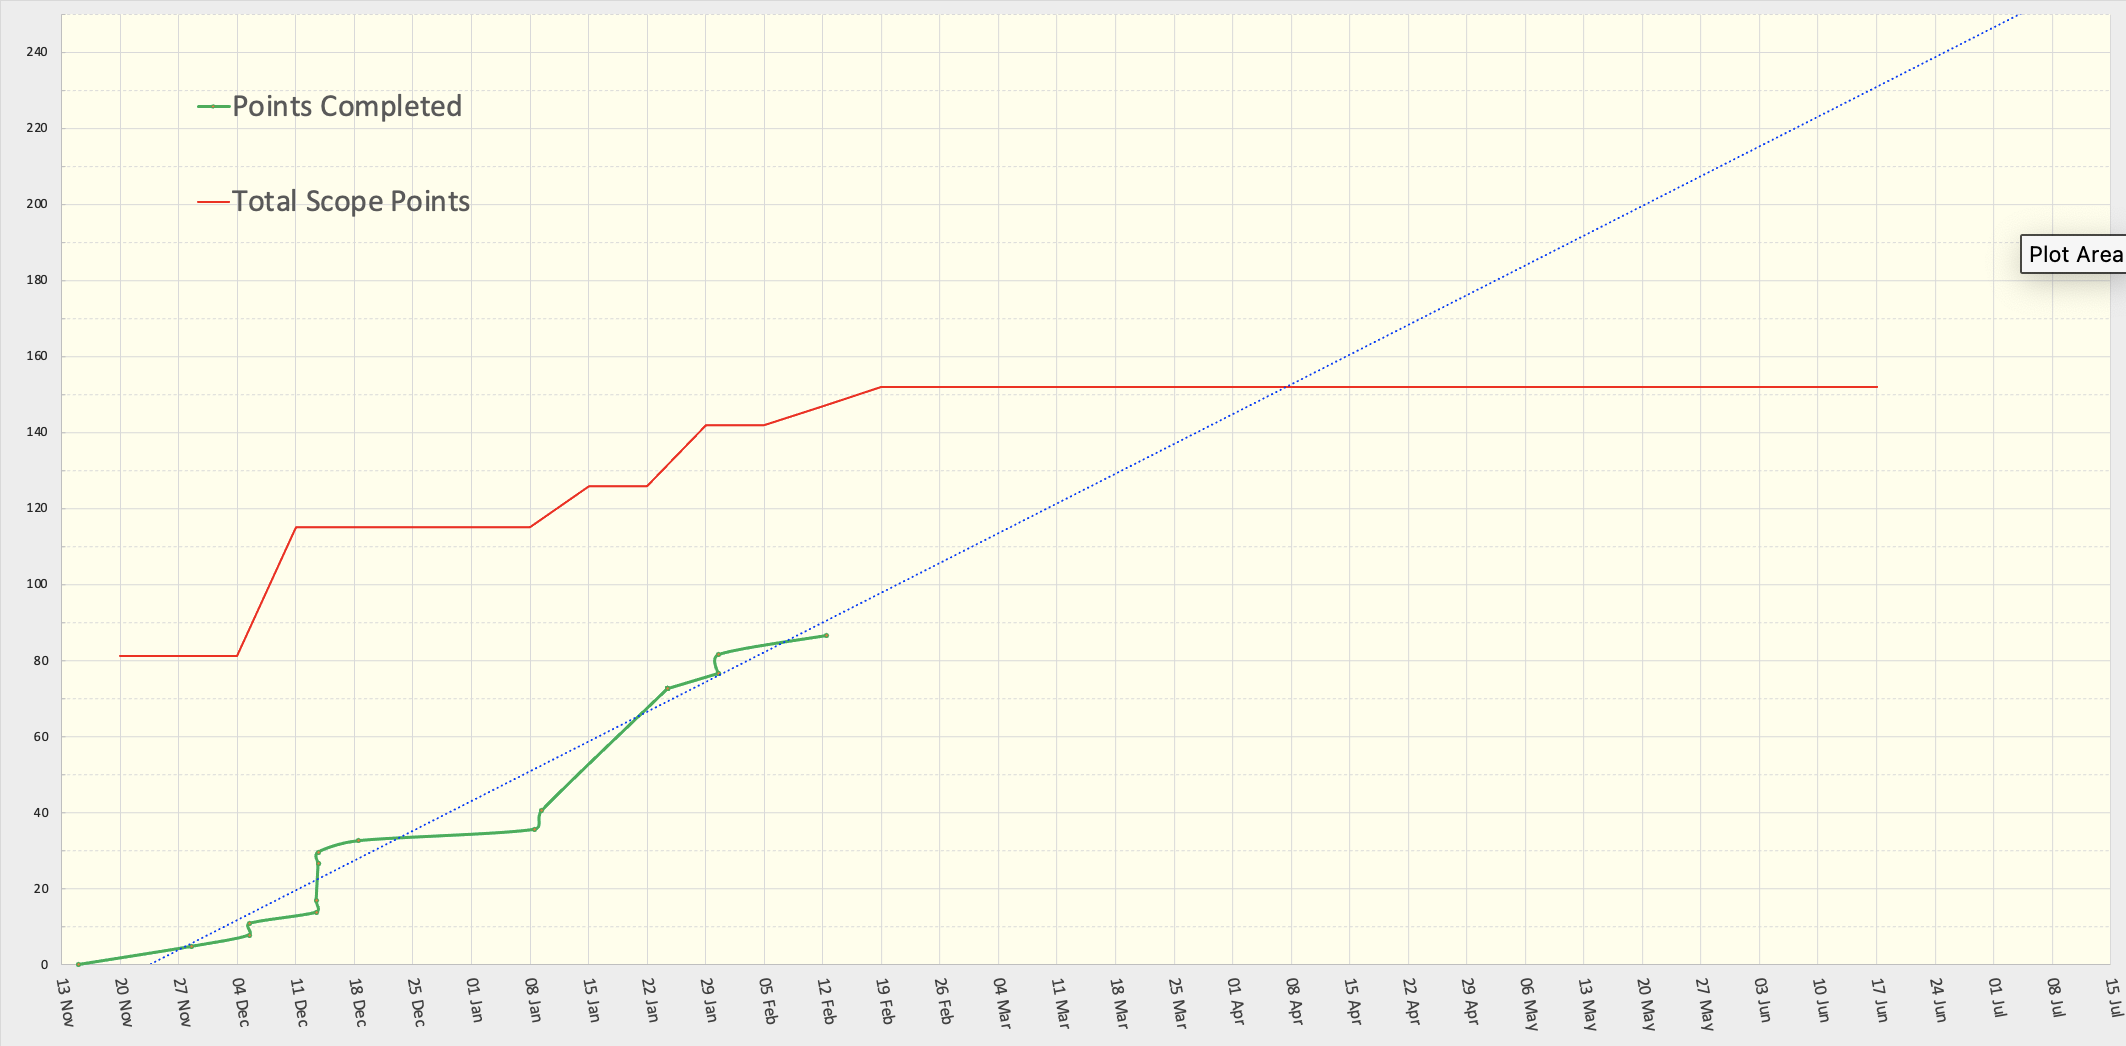
\includegraphics[width=12cm]{assets/outputs/burnups/02-14.png}
      \caption{Burn-up chart February 14th.}
      \label{fig:burnup4}
    \end{figure}
  
    \begin{figure}[H]
      \centering
      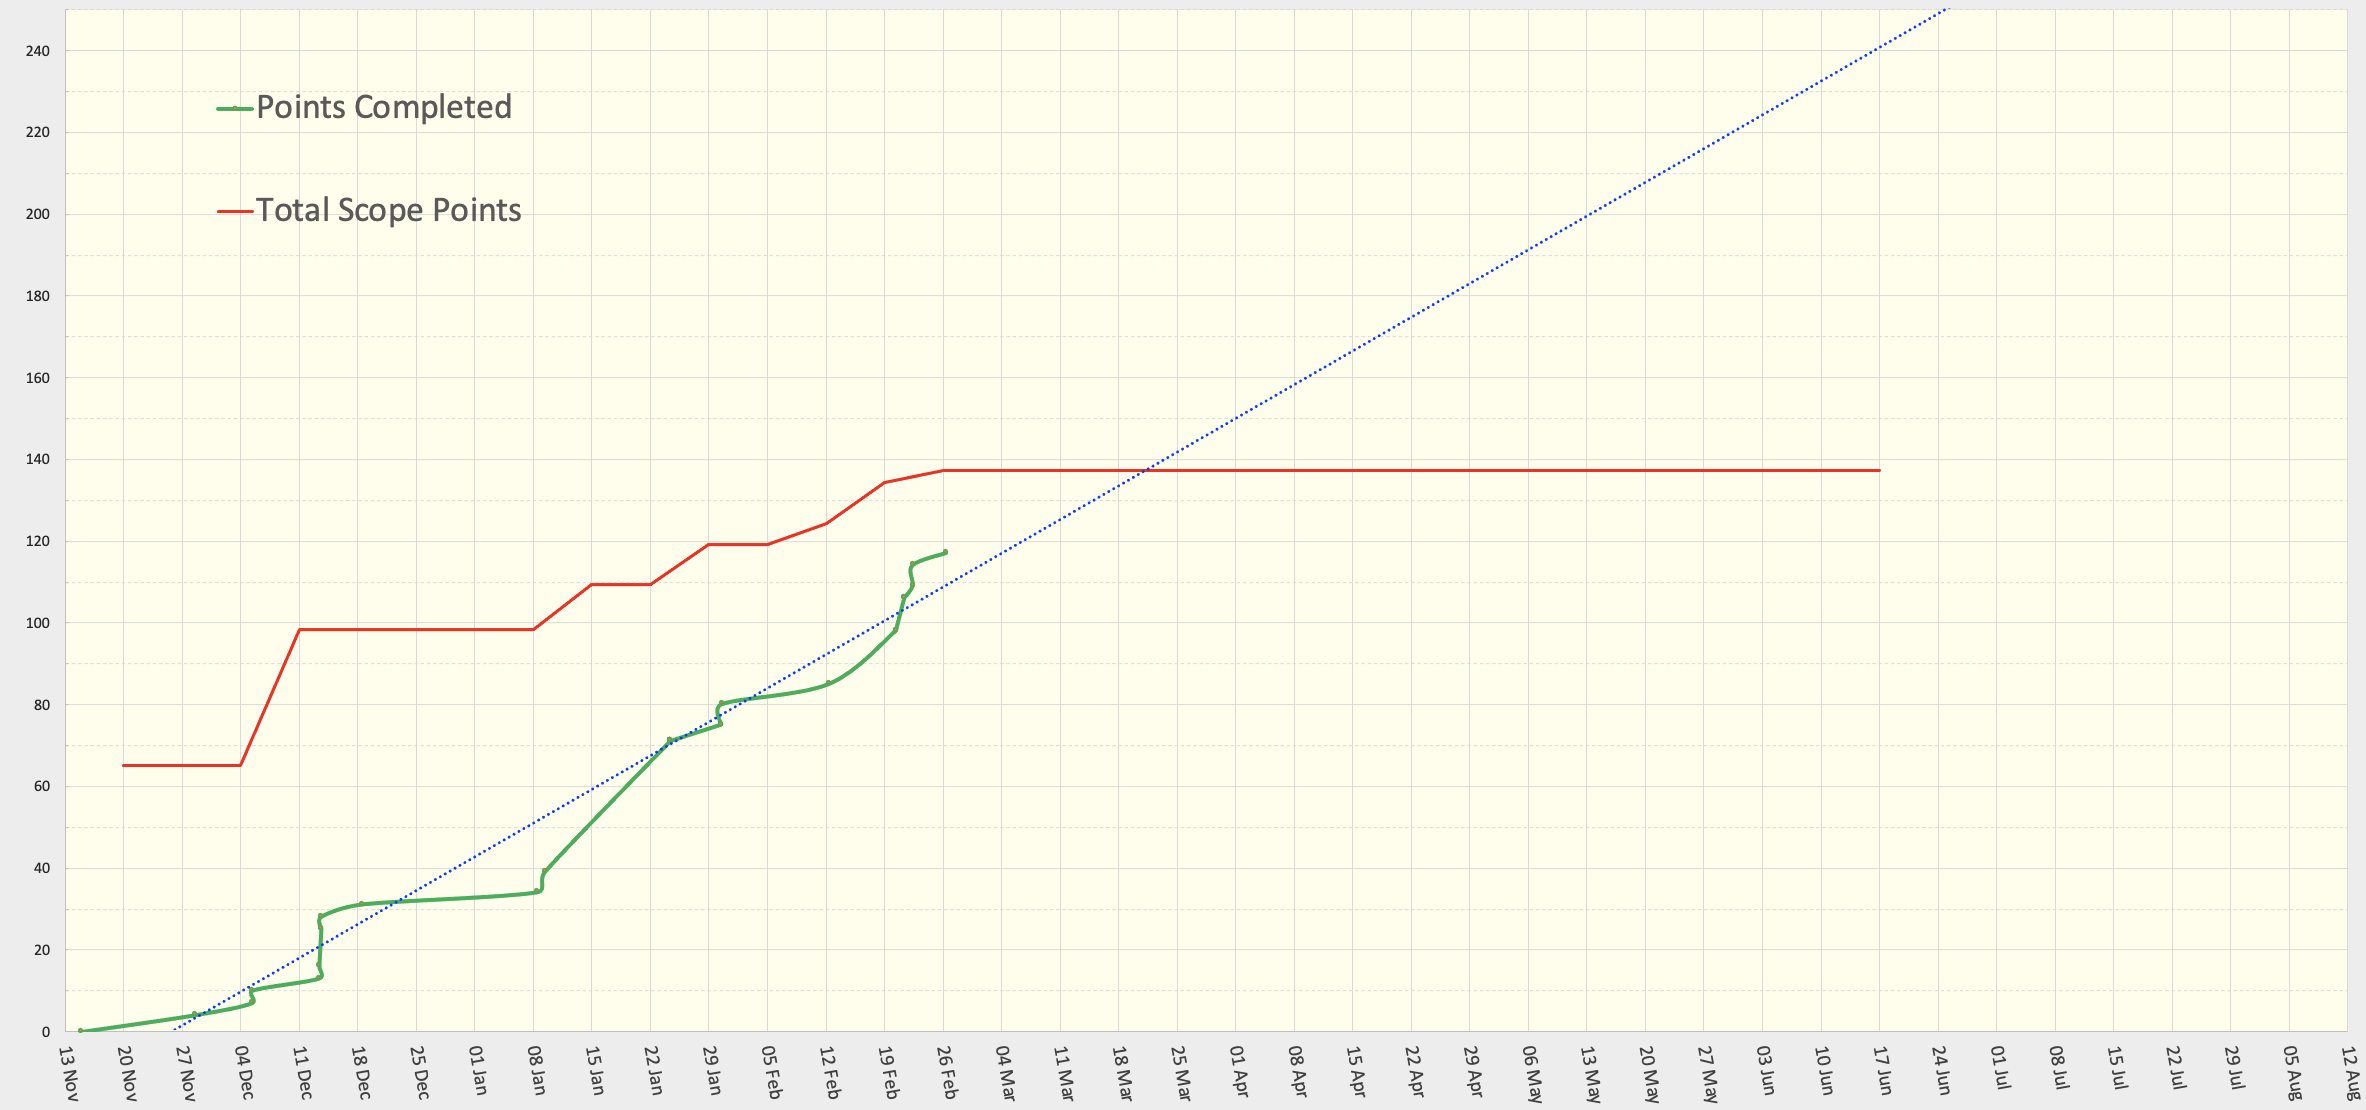
\includegraphics[width=12cm]{assets/outputs/burnups/02-27.png}
      \caption{Burn-up chart February 27th.}
      \label{fig:burnup5}
    \end{figure}
  
    \begin{figure}[H]
      \centering
      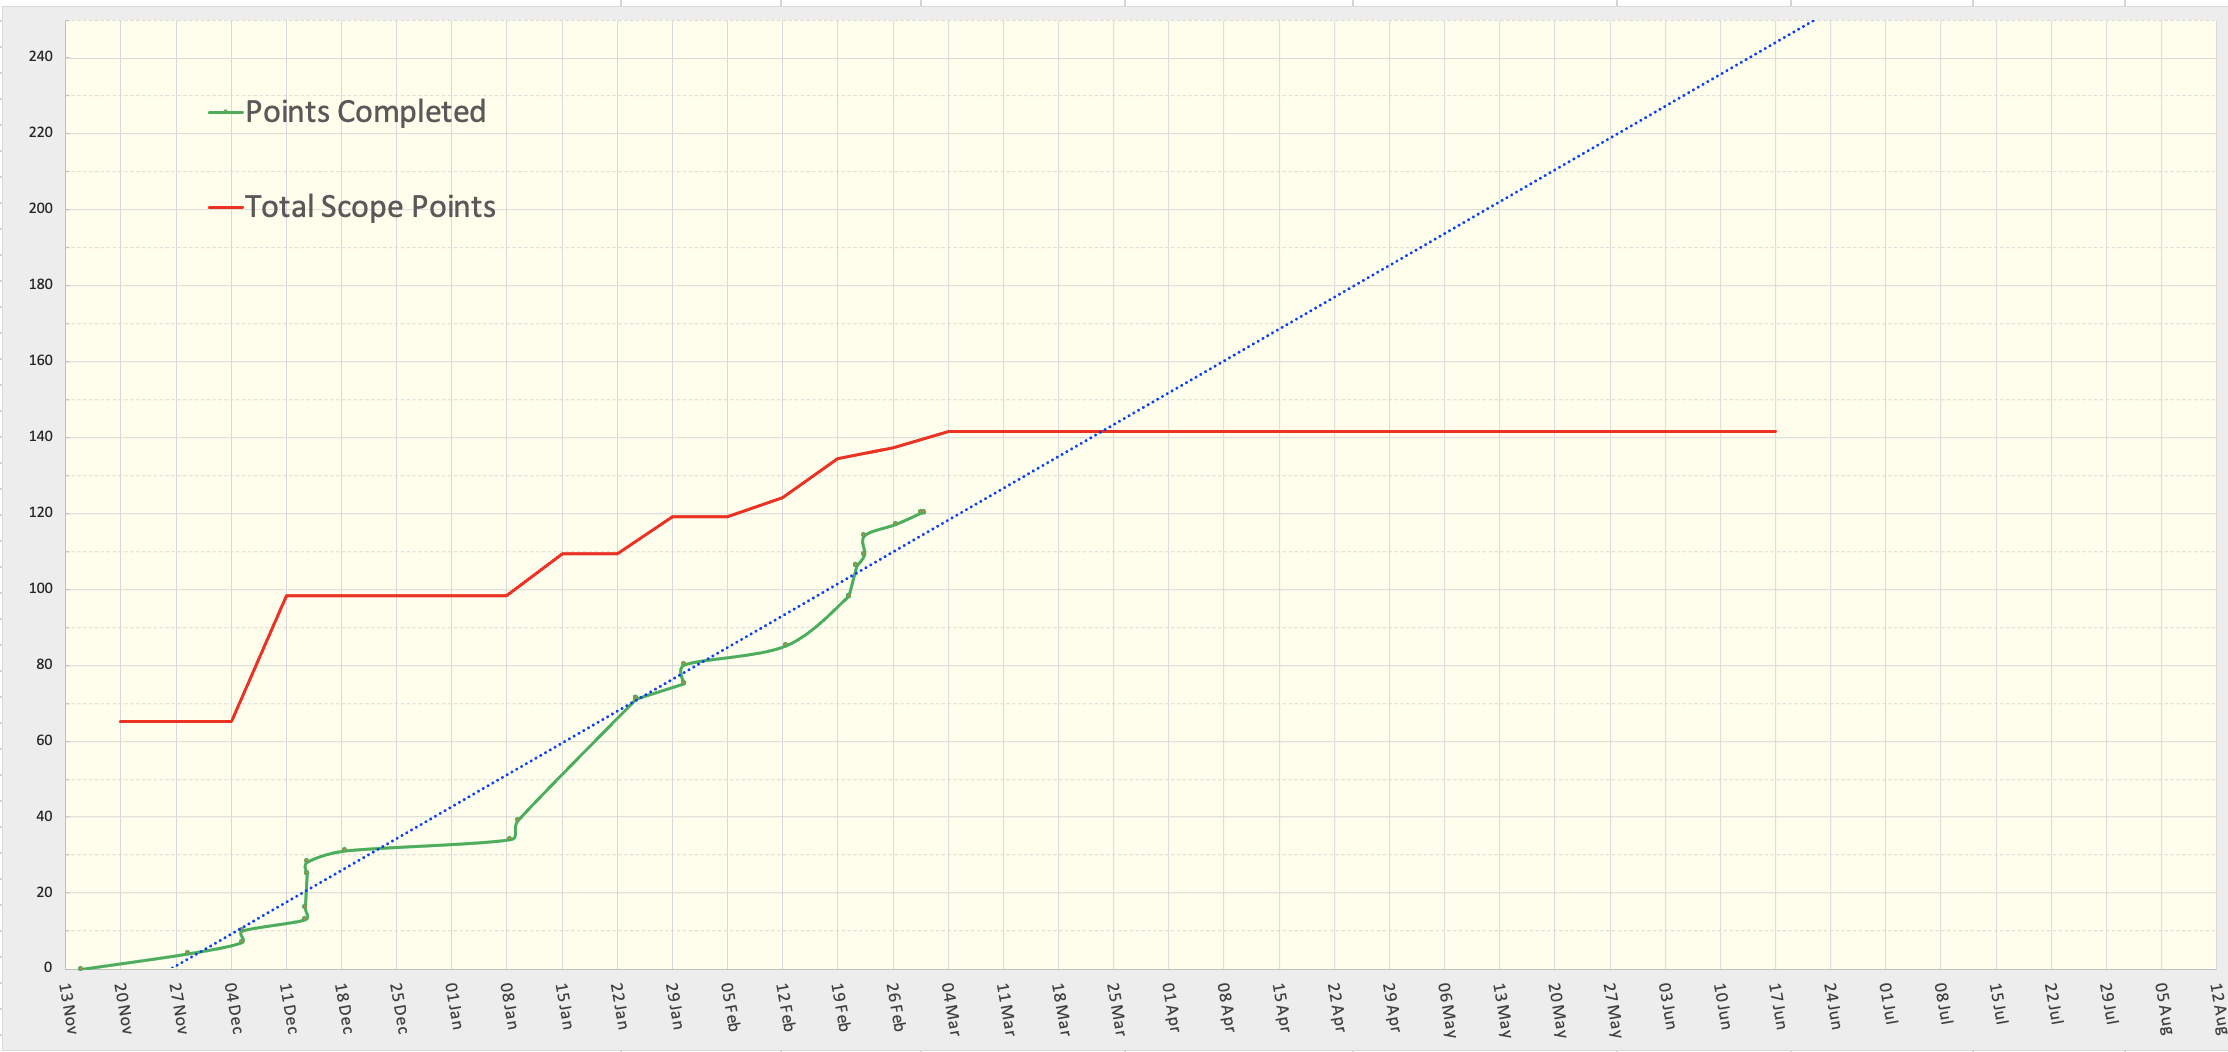
\includegraphics[width=12cm]{assets/outputs/burnups/03-03.png}
      \caption{Burn-up chart March 3rd.}
      \label{fig:burnup6}
    \end{figure}
  

  \newpage
  \subsection{Appendix H - Word Count}
  Total word count minus captions, tables, footnotes, references, appendix and indices \textbf{10,893}. 
  
  \newpage
  \subsection{Appendix I - Competency Mappings}
    \begin{longtable}{|p{2cm}|p{8cm}|p{4cm}|}
      \hline
      \textbf{Competency} & \textbf{Description} & \textbf{Page} \\ \hline
      B1                  & Identify, document, review, and design complex IT-enabled business
                            processes that define a set of activities that will accomplish specific
                            organisational goals and that provide a systematic approach to im-
                            proving those processes. & Pages 12 and 24 \\ \hline

      P3                  & Professionally present digital-and-technology-solution-specialism plans
                            and solutions in a well- structured business report. 
                            
                          & A viva was done as part of this module where the project was presented to a supervisor, line manager, independent
                          academic and senior manager from my company. \\ \hline

      P4                  & Demonstrate self-direction and originality in solving problems, and
                            act autonomously in planning and implementing digital-and-technology-
                            solution-specialist tasks at a professional level. & Pages 28 and 60 \\ \hline

      P5                  & Be competent at negotiating and closing techniques in a range of
                            interactions and engagements, both with senior internal stakeholders
                            and external stakeholders. & Pages 26, 28 and 46 \\ \hline

      SE-S01              & Architect, build, and support leading-edge concurrent-software plat-
                            forms that are performant to industry standards and that deliver
                            responsive solutions with good test coverage. & Pages 24, 45 and 47 \\ \hline

      SE-S02              & Drive the technology-decision-making and development process for
                            projects of varying scales, considering current technologies including
                            DevOps and Cloud Computing, and evaluate different technology-
                            design and implementation options, making reasoned proposals and
                            recommendations. & Page 28 \\ \hline

      SE-S03              & Develop and deliver distributed or semi-complex software solutions
                            that are scalable, and that deliver innovative user experiences and
                            journeys that encompass cross-functional teams, platforms, and technologies. & Page 52 \\ \hline

      SE-S04              & Update current software products, improving their efficiency and
                            functionality, and build new features to product specifications. 
                          
                          & This project is an upgrade to an existing component and these upgrades will improve the data we provide to partners 
                          by having our stores as up to date as is possible.  \\ \hline

      SE-S05              & Accomplish planned software-development tasks that deliver the expected
                            features within specified time constraints, security, and quality requirements. & Pages 47 and 50 \\ \hline

      SE-S06              & Be accountable for the quality of deliverables from one or more
                            software-development teams (source code quality, automated testing,
                            design quality, documentation, etc.), and following company-
                            standard processes (code reviews, unit testing, source code management, etc.)  & Pages 24 and 55 \\ \hline

      SE-K02              & The various inputs, statements of requirements, security considerations
                            and constraints that guide solution architecture and the development
                            of logical and physical systems' designs. & Pages 15, 26 and 47 \\ \hline

      SE-K03              & The methodologies designed to help create approaches for organizing
                            the software-engineering process, the activities that need to be
                            undertaken at different stages in the life-cycle, and techniques for
                            managing risks in delivering software solutions. & Pages 24 and 48 \\ \hline

      SE-K04              & The approaches used to modularise the internal structure of an
                            application, and to describe the structure and behaviour of applications
                            used in a business, with a focus on how they interact with each other
                            and with business users. & Pages 36, 39 and 58 \\ \hline

      SE-K05              & How to design, develop, and deploy software solutions that are secure
                            and effective in delivering the requirements of stakeholders, and
                            the factors that affect the design of a successful code. & Pages 24 and 55 \\ \hline

      SE-K06              & The range of metrics which might be used to evaluate a delivered
                            software product. & Pages 50 and 54 \\ \hline

      
    \end{longtable}